\subsection{Definition of the $\chi$ Field}
  \label{subsec:definition-of-the-chi-field}

  We postulate the existence of a single pre-geometric relational substrate, denoted $\chi$,
  which constitutes the primitive ontological basis of physical reality.
  The quantity $\chi$ is not defined on a pre-existing spacetime manifold and does not
  presuppose any metric, causal, or geometric structure.
  Instead, spacetime notions arise only as effective descriptions of the relational,
  spectral, and dynamical properties of $\chi$ configurations.

  Ontologically, $\chi$ is not a scalar order parameter and does not possess local values.
  Scalar order parameters arise only at the effective level, as coarse-grained descriptors
  of projected $\chi$ configurations once a geometric regime is established.
  Dimensional quantities associated with length, duration, or mass arise only at the
  effective level, when $\chi$ configurations admit a stable geometric interpretation.
  The monotonic ordering intrinsic to $\chi$ configurations gives rise, upon projection,
  to what is operationally perceived as temporal flow.

  \begin{tcolorbox}[colback=white, colframe=blue!75!black, title=Ontological Status of $\chi$]
    The $\chi$ substrate is \textbf{not}:
    \begin{itemize}
      \item A scalar field on spacetime (no background manifold).
      \item A dynamical degree of freedom (no time evolution at fundamental level).
      \item A discrete lattice or graph (fully continuous).
    \end{itemize}
    It is a \textbf{pre-geometric relational structure} from which spacetime, matter, and dynamics emerge via projection.
  \end{tcolorbox}

  Temporal ordering emerges from the global, irreversible ordering intrinsic to $\chi$
  configurations across physical processes, establishing an intrinsic arrow of time
  without reference to an external temporal coordinate.
  Spatial separation, in turn, arises from relational differences between $\chi$
  configurations, giving rise to an effective notion of distance once a quasi-stable
  geometric regime is reached.
  In this sense, time corresponds to ordering, while space corresponds to relational
  structure.

  At no stage is $\chi$ interpreted as a spacetime coordinate, as a physical field
  propagating on spacetime, or as a conventional dynamical variable.
  Spacetime coordinates and metric structure appear only as secondary, coarse-grained
  constructs, becoming meaningful when $\chi$ configurations admit a quasi-stable
  geometric interpretation through a generally non-injective projection.
  The spacetime metric thus functions as an emergent effective descriptor of resistance
  to $\chi$ relaxation\footnote{The term ``relaxation'' is used here in a geometric and
dynamical sense, and should not be confused with thermodynamic relaxation processes
involving dissipation or entropy increase.} and of the constrained propagation of
  perturbations within the projected description.

  The analogy with thermodynamic order parameters applies only at the effective level:
  $\chi$ itself is not an order parameter, but gives rise to effective order parameters
  once projected.
  Within the Cosmochrony framework, $\chi$ therefore provides the minimal ontological
  substrate from which time, space, inertial mass, gravitation, and quantum phenomena
  jointly emerge as harmonics of a single irreversible relaxation process.

  In the following sections, spacetime coordinates, metric quantities, and field-theoretic
  objects will be introduced strictly as effective tools, valid only in regimes where
  $\chi$ admits a stable geometric interpretation.

  \begin{figure}[h]
    \centering
    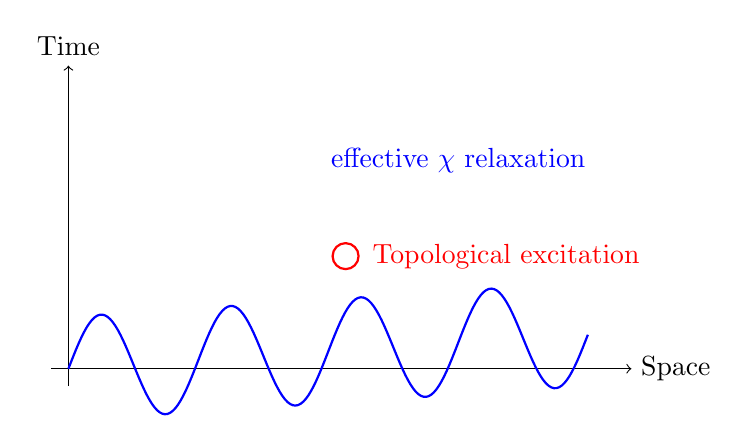
\begin{tikzpicture}[scale=1.1]

% Axes
      \draw[->] (-0.2,0) -- (6.5,0) node[right]{Space};
      \draw[->] (0,-0.2) -- (0,3.5) node[above]{Time};

% Wave
      \draw[thick, blue, domain=0:6, samples=200]
      plot (\x,{0.6*sin(2*pi*\x/1.5 r) + 0.4*\x/6});

% Particle crest
      \draw[red, thick] (3.2,1.3) circle (0.15);
      \node[red, right] at (3.4,1.3) {Topological excitation};

% Annotation
      \node[blue] at (4.5,2.4) {effective $\chi$ relaxation};

    \end{tikzpicture}
    \caption{Conceptual representation of Cosmochrony.
    An effective spacetime depiction of the projected scalar description of $\chi$,
      used for visualization purposes only.
      The monotonic relaxation of $\chi$ gives rise to an effective temporal ordering,
      while localized topological excitations correspond to particle-like configurations
      in the emergent geometric regime.}
    \label{fig:chi_concept}
  \end{figure}

  \paragraph{On the use of spacetime language.}
    Throughout this work, phrases such as ``spacetime coordinates,'' ``metric tensor,''
    and ``four-dimensional manifold'' are employed for clarity and effective description.
    These notions should be understood strictly as \emph{emergent, projected constructs}
    valid only in regimes where $\chi$ has relaxed into a quasi-stable geometric
    configuration.
    They do not correspond to fundamental ingredients of the theory.

    At the most fundamental level, only $\chi$ and its internal relational and spectral
    structure exist.
    The appearance of familiar geometric language reflects the effectiveness of spacetime
    as a coarse-grained description of collective $\chi$ behavior, analogous to how
    thermodynamic variables (such as temperature or pressure) emerge from molecular
    dynamics without being fundamental.

    This interpretational stance is essential for distinguishing Cosmochrony from
    approaches that merely reformulate existing geometric theories in alternative
    variables, rather than addressing the physical origin of geometry itself.

    Extended interpretative clarifications, including common misreadings and the
    status of field-theoretic notation, are provided in
    Appendix~\ref{subsec:nature-chi}.
    The fully relational formulation of $\chi$ configurations, independent of
    geometric or manifold structures, is developed in
    Appendix~\ref{subsec:relational-configurations-of-chi}.
